
\documentclass[
% -- opções da classe memoir --
12pt,				% tamanho da fonte
openright,			% capítulos começam em pág ímpar (insere página vazia caso preciso)
oneside,			% para impressão em recto e verso. Oposto a oneside
a4paper,			% tamanho do papel. 
% -- opções da classe abntex2 --
chapter=TITLE,		% títulos de capítulos convertidos em letras maiúsculas
section=TITLE,		% títulos de seções convertidos em letras maiúsculas
%subsection=TITLE,	% títulos de subseções convertidos em letras maiúsculas
%subsubsection=TITLE,% títulos de subsubseções convertidos em letras maiúsculas
% -- opções do pacote babel --
english,			% idioma adicional para hifenização
french,				% idioma adicional para hifenização
spanish,			% idioma adicional para hifenização
brazil				% o último idioma é o principal do documento
]{abntex2-uepg}

% ---
% Pacotes básicos 
% ---
\usepackage{lmodern}			% Usa a fonte Latin Modern			
\usepackage[T1]{fontenc}		% Selecao de codigos de fonte.
\usepackage[utf8]{inputenc}		% Codificacao do documento (conversão automática dos acentos)
\usepackage{indentfirst}		% Indenta o primeiro parágrafo de cada seção.
\usepackage{color}				% Controle das cores
\usepackage{graphicx}			% Inclusão de gráficos
\usepackage{microtype} 			% para melhorias de justificação]
\usepackage{uepg}
\usepackage{lipsum}		
\usepackage{amssymb}
\usepackage{amsmath}
%\usepackage{paralist}
\usepackage{setspace}
\usepackage{lscape}
\usepackage{longtable}	
\usepackage{listings}
\usepackage{gantt}
\usepackage{inconsolata}
\usepackage{xcolor}
\usepackage[bottom=2cm,top=3cm,left=3cm,right=2cm]{geometry}
\usepackage{titlesec}
\titlespacing*{\subsection}{0pt}{2.5ex plus 1ex minus .2ex}{2.5ex plus .2ex} 

\setlength\afterchapskip{\lineskip}

\definecolor{codegreen}{rgb}{0,0.6,0}
\definecolor{codegray}{rgb}{0.5,0.5,0.5}
\definecolor{codepurple}{rgb}{0.58,0,0.82}
\definecolor{backcolour}{rgb}{0.95,0.95,0.92}

\lstdefinestyle{mystyle}{
	backgroundcolor=\color{backcolour},   
	commentstyle=\color{codegreen},
	keywordstyle=\color{magenta},
	numberstyle=\tiny\color{codegray},
	stringstyle=\color{codepurple},
	basicstyle=\ttfamily\footnotesize,
	breakatwhitespace=false,         
	breaklines=true,                 
%	captionpos=b,                    
	keepspaces=true,                 
	numbers=left,                    
	numbersep=5pt,                  
	showspaces=false,                
	showstringspaces=false,
	showtabs=false,                  
	tabsize=2,
	frame=single
}

\lstset{style=mystyle}

\usepackage[brazilian,hyperpageref]{backref}	 % Paginas com as citações na bibl
\usepackage[alf,
abnt-emphasize = bf, % destaca o titulo da revista ou livro em negrito;
abnt-etal-list = 3, % trabalhos com mais de 3 autores recebem et al.,;
abnt-etal-text = it, % escreve o et al., em italico;
abnt-and-type = &, % usa o carater '&' no lugar de 'e' para mais de um autor;
abnt-last-names = abnt, % trata sobrenomes 'estritamente' conforme a ABNT; e
abnt-repeated-author-omit = no % autores com + de uma entrada recebem '____.'
]{abntex2cite}

% ---
% Configurações do pacote backref
% Usado sem a opção hyperpageref de backref
\renewcommand{\backrefpagesname}{Citado na(s) página(s):~}
% Texto padrão antes do número das páginas
\renewcommand{\backref}{}
% Define os textos da citação
\renewcommand*{\backrefalt}[4]{
	\ifcase #1 %
	Nenhuma citação no texto.%
	\or
	Citado na página #2.%
	\else
	Citado #1 vezes nas páginas #2.%
	\fi}%
% ---
% -- ljsenger
\renewcommand{\rmdefault}{phv} % Arial
\renewcommand{\sfdefault}{phv} % Arial

% formatacao de codigo fonte
\renewcommand{\lstlistingname}{Código}
\renewcommand{\lstlistlistingname}{Lista de códigos}

% ---
% Informações de dados para CAPA e FOLHA DE ROSTO
% ---
\titulo{Formatação de trabalhos para a UEPG com o uso da classe \abnTeX}% \titulo{Formatação de trabalhos para a UEPG com o uso da classe \abnTeX}
\autor{Seu Nome Aqui} 
\local{Brasil}
\data{Outono de 2021}
\orientador{Nome do orientador}
\coorientador{Equipe \abnTeX}

	
\tipotrabalho{Trabalho de Conclusão de Curso}
% O preambulo deve conter o tipo do trabalho, o objetivo, 
% o nome da instituição e a área de concentração 
\preambulo{Trabalho de conclusão de Curso apresentado como requisito parcial para obtenção do
	título de Bacharel em Engenharia de Computação na Universidade Estadual de Ponta Grossa}

\definecolor{blue}{RGB}{41,5,195}

\makeatletter
\hypersetup{
	%pagebackref=true,
	pdftitle={\@title}, 
	pdfauthor={\@author},
	pdfsubject={\imprimirpreambulo},
	pdfcreator={LaTeX with abnTeX2},
	pdfkeywords={abnt}{latex}{abntex}{abntex2}{trabalho acadêmico}, 
	colorlinks=true,       		% false: boxed links; true: colored links
	linkcolor=black,          	% color of internal links
	citecolor=black,        		% color of links to bibliography
	filecolor=magenta,      		% color of file links
	urlcolor=black,
	bookmarksdepth=4
}
\makeatother
% --- 

% ---
% Posiciona figuras e tabelas no topo da página quando adicionadas sozinhas
% em um página em branco. Ver https://github.com/abntex/abntex2/issues/170
\makeatletter
\setlength{\@fptop}{5pt} % Set distance from top of page to first float
\makeatother
% ---

% ---
% Possibilita criação de Quadros e Lista de quadros.
% Ver https://github.com/abntex/abntex2/issues/176
%
\newcommand{\quadroname}{Quadro}
\newcommand{\listofquadrosname}{Lista de quadros}

\newfloat[chapter]{quadro}{loq}{\quadroname}
\newlistof{listofquadros}{loq}{\listofquadrosname}
\newlistentry{quadro}{loq}{0}


% configurações para atender às regras da ABNT
\setfloatadjustment{quadro}{\centering}
\counterwithout{quadro}{chapter}
\renewcommand{\cftquadroname}{\quadroname\space} 
\renewcommand*{\cftquadroaftersnum}{\hfill--\hfill}

\setfloatlocations{quadro}{hbtp} % Ver https://github.com/abntex/abntex2/issues/176
% ---

% --- 
% Espaçamentos entre linhas e parágrafos 
% --- 

% O tamanho do parágrafo é dado por:
\setlength{\parindent}{1.3cm}

% Controle do espaçamento entre um parágrafo e outro:
\setlength{\parskip}{0.2cm}  % tente também \onelineskip

%ljsenger - espaçamento simples (e feio) entre parágrafos
\setlength{\parskip}{0cm}
%ljsenger - espaçamento entre o título e o primeiro parágrafo do texto
\setlength\afterchapskip{18pt}

% compila o indice
\makeindex
% ---
% padrão UEPG - fonte ARIAL (ou times)
\renewcommand{\rmdefault}{phv} % Arial
\renewcommand{\sfdefault}{phv} % Arial

\newlistof{lstlistoflistings}{lol}{\lstlistlistingname}
\begin{document}
	
	\selectlanguage{brazil}
	\frenchspacing 
	
	\imprimircapa
	% ---
	
	% ---
	% Folha de rosto
	% (o * indica que haverá a ficha bibliográfica)
	% ---
	\imprimirfolhaderosto
	
	% ---
	% Dedicatória
	% ---
	\begin{dedicatoria}
		\vspace*{\fill}
		\centering
		\noindent
		\textit{ Dedico esta monografia  à minha professora orientadora que me manteve focado e na trilha certa para a conclusão satisfatória deste projeto. Grato pela sua orientação preciosa..} \vspace*{\fill}
	\end{dedicatoria}
	
	\begin{agradecimentos}
		Este documento utiliza a classe abntex, seguem os agradecimentos para os criadores do pacote. Os agradecimentos principais são direcionados à Gerald Weber, Miguel Frasson,
Leslie H. Watter, Bruno Parente Lima, Flávio de Vasconcellos Corrêa, Otavio Real
Salvador, Renato Machnievscz\footnote{Os nomes dos integrantes do primeiro
	projeto abn\TeX\ foram extraídos de
	\url{http://codigolivre.org.br/projects/abntex/}} e todos aqueles que
contribuíram para que a produção de trabalhos acadêmicos conforme
as normas ABNT com \LaTeX\ fosse possível.

Agradecimentos especiais são direcionados ao Centro de Pesquisa em Arquitetura
da Informação\footnote{\url{http://www.cpai.unb.br/}} da Universidade de
Brasília (CPAI), ao grupo de usuários
\emph{latex-br}\footnote{\url{http://groups.google.com/group/latex-br}} e aos
novos voluntários do grupo
\emph{\abnTeX}\footnote{\url{http://groups.google.com/group/abntex2} e
	\url{http://www.abntex.net.br/}}~que contribuíram e que ainda
contribuirão para a evolução do \abnTeX.
		
	\end{agradecimentos}
	% ---
	
	% ---
	% Epígrafe
	% ---
	\begin{epigrafe}
	\vspace*{\fill}
	\begin{flushright}
		\textit{"A menos que modifiquemos a nossa maneira de pensar,\\ não seremos capazes de resolver os problemas causados \\ pela forma como nos acostumamos a ver o mundo". (Albert Einstein)}
	\end{flushright}
\end{epigrafe}
	\setlength{\absparsep}{18pt} % ajusta o espaçamento dos parágrafos do resumo
	\begin{resumo}
			Segundo a \citeonline[3.1-3.2]{NBR6028:2003}, o resumo deve ressaltar o
objetivo, o método, os resultados e as conclusões do documento. A ordem e a extensão
destes itens dependem do tipo de resumo (informativo ou indicativo) e do
tratamento que cada item recebe no documento original. O resumo deve ser
precedido da referência do documento, com exceção do resumo inserido no
próprio documento. (\ldots) As palavras-chave devem figurar logo abaixo do
resumo, antecedidas da expressão Palavras-chave:, separadas entre si por
ponto e finalizadas também por ponto.

\textbf{Palavras-chave}: latex. abntex. editoração de texto.
	\end{resumo}
	
	% resumo em inglês
	%\begin{resumo}[Abstract]
	%	\begin{otherlanguage*}{english}
	%		Este é o abstract do trabalho. Lembre-se que conforme o modelo da UEPG, o abstract não é obrigatório para trabalhos de conclusão de Curso, mas é obrigatório para dissertações de mestrado e doutorado. 
			
	%		\vspace{\onelineskip}
			
	%		\noindent 
	%		\textbf{Keywords}: latex. abntex. text editoration.
	%	\end{otherlanguage*}
	%\end{resumo}
	
	% inserir lista de ilustrações
	% ---
	\renewcommand{\listfigurename}{Lista de figuras}
	\pdfbookmark[0]{\listfigurename}{lof}
	\listoffigures*
	\cleardoublepage
	% inserir lista de quadros
	% ---
	\pdfbookmark[0]{\listofquadrosname}{loq}
	\listofquadros*
	\cleardoublepage
	% inserir lista de tabelas
	% ---
	\pdfbookmark[0]{\listtablename}{lot}
	\listoftables*
	\cleardoublepage
	% inserir lista de abreviaturas e siglas
	% ---
	%\pdfbookmark[0]{\lstlistlistingname}{lot}
	\lstlistoflistings*
	\cleardoublepage
	% inserir lista de abreviaturas e siglas
	\begin{siglas}
		\item[ABNT] Associação Brasileira de Normas Técnicas
\item[UEPG] Universidade Estadual de Ponta Grossa
\item[LCAD] Laboratório de Computação de Alto Desempenho
	\end{siglas}
	% ---
	
	% ---
	% inserir lista de símbolos
	% ---
	\begin{simbolos}
		\item[$ \Gamma $] Letra grega Gama
\item[$ \Lambda $] Lambda
\item[$ \zeta $] Letra grega minúscula zeta
\item[$ \in $] Pertence
	\end{simbolos}
	% ---
	
	% ---
	% inserir o sumario
	% ---
	\pdfbookmark[0]{\contentsname}{toc}
	\tableofcontents*
	\cleardoublepage
	% ----------------------------------------------------------
	\textual
	
	\chapter{Introdução}
Este trabalho utiliza o pacote abntex~\cite{abntex2classe}. 
Edite o arquivo uepg.sty para incluir dados sobre a instituição (setor de conhecimento e departamento).

Edite o arquivo tcc.tex para incluir os arquivos de sua dissertação. Os arquivos que são incluídos estão listados abaixo:

\begin{itemize}	
	\item introducao
	\item revisao
 	\item metodologia
	\item resultados
	\item conclusao
\end{itemize}

Você pode incluir mais arquivos editando o tcc.tex, caso sua dissertação necessite de mais capítulos.

Edite os arquivos siglas.tex, simbolos.tex e resumo.tex para incluir o texto de sua dissertação.


	\chapter{Revisão da Literatura}
\citeonline{Moh06} desenvolveram um trabalho utilizando MD no qual o objetivo foi desenvolver modelos para classificação de doenças do arroz egípcio. Um dos algoritmos de aprendizagem utilizado foi a RNA. A RNA foi construída e treinada utilizando uma configuração de 52 entradas, 33 neurônios na camada oculta, 5 saídas, taxa de aprendizagem de 0.3, momento de 0.2 e 500 iterações. O modelo obtido para a previsão de doenças de arroz atingiu um índice de acerto de 96,4\% para o conjunto de dados de teste. Este resultado demonstra a grande eficiência da aplicação de RNAs.

O processo de mineração de dados é ilustrado na Figura~\ref{fig:mineracao}.
\begin{figure}
	\centering
	\caption{Etapas da mineração de dados}\label{fig:mineracao}
	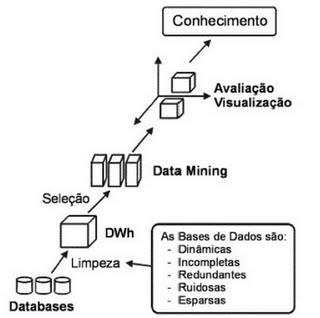
\includegraphics[scale=1.0]{mineracao}
	
\end{figure}



	\chapter{Material e Métodos}
\section {Considerações Iniciais}
A partir da classe com menor representatividade na base de dados, classe 4 - Algodão Americano/Salgueiro com 2.747 observações, sendo todos os dados selecionados, foram extraídas das outras seis classes de tipos de cobertura florestal 2.747 observações, selecionadas aleatoriamente com o auxilio do software R, totalizando o conjunto de teste com 19.229 observações, conforme a tabela \ref{tb:dados}.
\subsection[Teste de subseção]{ Teste de subseção}
\begin{table}[htbp]
\caption{Observações Selecionadas}
\label{tb:dados}
\centering
\setlength{\tabcolsep}{5pt}
\begin{tabular}{cccccc}
\hline
Tipo de Cobertura  &Total de  &Observações  &Porcentagem por \\
Florestal &Observações &Selecionadas &Tipo de Cobertura \\
\hline
Classe 1 &211.840 &2747 &1,29\% \\
Classe 2 &283.301 &2747 &0,97\% \\
Classe 3 &35.754  &2747 &7,68\% \\
Classe 4 &2.747   &2747 &100\% \\
Classe 5 &9.493   &2747 &28,94\% \\
Classe 6 &17.367  &2747 &15,82\% \\
Classe 7 &20.510  &2747 &13,39\% \\
\hline
\textbf{Total} &\textbf{581.012} &\textbf{19.229} &\textbf{3,31\%} \\
\hline
\end{tabular}
\\
%\singlespacing
%\text{\footnotesize Fonte: O autor}
\end{table}

\section{Exemplo de Código Fonte}
O código~\ref{code:oddoreven} apresenta um exemplo de uso de listagem de código.

%\lstset{frame=Trbl,numbers=left}
\begin{lstlisting}[caption={Exemplo de código fonte}, language=Python, label=code:oddoreven]
	# Python program to check if the input number
	# is odd or even.
	# A number is even if division by 2 gives a
	# remainder of 0.
	# If the remainder is 1, it is an odd number.
	
	num = int(input("Enter a number: "))
	if (num % 2) == 0:
		print("{0} is Even".format(num))
	else:
		print("{0} is Odd".format(num))
\end{lstlisting}	


\section{Análise dos Dados}


\section{Cronograma}
Visando atingir os objetivos propostos apresenta-se um cronograma
de atividades a ser realizado. Estas atividades e o cronograma
estão ilustrados nas tabelas \ref{tb:atividades} e
\ref{fig:cronograma}, respectivamente.


\begin{table}[!htb]
	\centering
	\caption{Atividades Previstas}\label{tb:atividades}
	\begin{tabular}{cp{12cm}}
		\hline \hline &\\[-0.4cm]
		Atividades& \multicolumn{1}{c}{ Descrição} \\
		\hline
		&\\[-0.4cm]
		\textbf{A} & Revisão bibliográfica. \\[0.2cm]
		\textbf{B} &  Estudo de novas representações.\\[0.2cm]
		\textbf{C} &  Aplicação dos algoritmos.\\[0.2cm]
		\textbf{D} &  Desenvolvimento da interface. \\[0.2cm]
		\textbf{E} &  Validação dos resultados.\\[0.2cm]
		\textbf{F} &  Elaboração da monográfia.\\[0.2cm]
		\textbf{G} &  Defesa.\\[0.2cm]
		\hline \hline
	\end{tabular}
\end{table}

%\begin{preview}
%\centering

\begin{figure}
	\caption{Cronograma de Atividades}\label{fig:cronograma}
	\begin{gantt}{10}{12}
		\begin{ganttitle}
			\numtitle{1}{1}{12}{1}
		\end{ganttitle}
		\ganttbar{Revisão da literatura}{0}{2}
		\ganttbarcon{refinamento método}{2}{5}
		\ganttbarcon{}{8}{2}
		\ganttmilestone[color=cyan]{Milestone with color!}{4}
		\ganttbar{another task}{2}{2}
		\ganttbar[color=cyan]{another coloured task}{4}{4}
		\ganttbar{another task}{4}{2}
		\ganttcon{4}{5}{4}{7}
		\ganttmilestonecon{A connected Milestone}{7}
		\ganttbarcon{another consecutive task}{8}{2}
	\end{gantt}
	%\end{preview}
	
\end{figure}
\section{Recursos}
Descrever os recursos necessários para o desenvolvimento da pesquisa.
\subsection{Recursos Humanos}
\subsection{Recursos Físicos}

	\chapter{Resultados}

De maneira geral, a medida que aumenta-se o número de pares também aumenta a eficiência (Tabela~\ref{tab:p2p}). O \textit{rank} 0, que não realiza processamento, começa a representar uma porcentagem cada vez menor para o calculo da eficiência. Considerando 3 pares, o \textit{rank} 0 representa 33\% do calculo da eficiência, já considerando 5 pares o mesmo representa 20\%, assim a medida que aumentam-se os pares a eficiência aumenta. Está melhoria ocorre até certo ponto, pois a comunicação entre processos aumenta e medida que adicionamos novos pares. É importante ressaltar que esta particularidade ocorre devido ao \textit{rank} 0 não processar nenhuma atividade e participar do calculo de eficiência, e com o aumento do números de pares a eficiência diminua devido as taxas de comunicação. Se desconsiderado o \textit{rank} 0, a eficiência observada inicia elevada e na medida que aumentam-se os pares a eficiência deve diminuir devido à comunicação entre processos da rede.

\begin{table}[!h]
\caption{ Resumo dos resultados modo P2P - 10 \textit{Folds} }
\label{tab:p2p}
\centering
\setlength{\tabcolsep}{5pt}
\begin{tabular}{ccccccc}
\hline
Grupo &Grupo 1 &Grupo 2 &Grupo 3 &Grupo 4 &Grupo 5 &Grupo 6 \\
\hline
Experimento &Sequencial &3-Pares &5-Pares &7-Pares &9-Pares &11-Pares \\
\hline
Média &301,92 &146,07 &91,22 &61,44 &60,98 &31,97 \\
\hline
Desvio Padrão &1,05 &0,88 &1,10 &0,69 &0,75 &0,82 \\
\hline
\multicolumn{2}{c}{\textit{SpeedUp}} &2,07 &3,31 &4,91 &4,95 &9,44 \\
\hline
\multicolumn{2}{c}{Eficiência} &0,69 &0,66 &0,70 &0,55 &0,86 \\
\hline
\end{tabular}
%\\
%\singlespacing
%\text{\footnotesize Fonte: O autor}
\end{table}

	\chapter{Conclusão}
\setlength{\afterchapskip}{-\baselineskip}
\lipsum  

	
	\postextual
	%ljsenger - espaçamento entre o título e o primeiro parágrafo do texto
	\setlength\afterchapskip{18pt}
	%\bibliographystyle{abntex2-alf}
	\bibliography{base}

% ----------------------------------------------------------
% Glossário
% ----------------------------------------------------------
%
% Consulte o manual da classe abntex2 para orientações sobre o glossário.
%
%\glossary

% ----------------------------------------------------------
% Apêndices
% ----------------------------------------------------------

% ---
% Inicia os apêndices
% ---
\begin{apendicesenv}
	
	% Imprime uma página indicando o início dos apêndices
	%\partapendices
	
	\renewcommand{\thetable}{\Alph{chapter}\arabic{table}}
	\setcounter{table}{0}
	\clearpage
		\begingroup%
		\makeatletter%
		\let\clearpage\relax% Stop LaTeX from going to a new page; and
		\vspace*{\fill}%
		\vspace*{\dimexpr-50\p@-\baselineskip}% Remove the initial (default) 50pt gap (plus 1 line)
		\chapter{Análise Estatística}
		% inserir aqui o texto do apendice via \input{}
		\vspace*{\fill}%
		\endgroup 
	\clearpage

	% ----------------------------------------------------------
	
	\lipsum[50]
	
	
\end{apendicesenv}
% ---


% ----------------------------------------------------------
% Anexos
% ----------------------------------------------------------

% ---
% Inicia os anexos
% ---
\begin{anexosenv}
	
	% Imprime uma página indicando o início dos anexos
	%\partanexos
	
	% ---
	\chapter{Laudo técnico}
	% ---
	\lipsum[30]
		
\end{anexosenv}

%---------------------------------------------------------------------
% INDICE REMISSIVO
%---------------------------------------------------------------------
\phantompart
\printindex
%---------------------------------------------------------------------

\end{document}	